% STUDYGROUP/DUISC/STEM
% ASSIGNMENT REPORT TEMPLATE
% (c) Jeff Davidson 2020-10-28

% LOAD CUSTOM CLASS - DO NOT REMOVE THIS COMMAND
% serif fonts are required to meet IEEE standards and clearly render variables and equations
\documentclass{jmd_duisc_report} % computer modern (LaTeX default)
%\documentclass[tm]{jmd_duisc_report} % times

% PARAMETERS FOR THIS REPORT - COMPLETE AS REQUIRED
% these parameters are used to create the cover page, title page, headers and footers
\department{DUISC STEM}
\programmetitle{IFY Computer Science}
\moduletitle{Computer Science with Extended Research}
\tutorname{Chris Roberts}
\teachinggroup{JFSCS\_CSER}
\assignmentcode{F\_CSER\_J\_A2: }
\assignmenttitle{Project: Minimum Connector Problem}
\assignmentdeadline{30/07/2021}
\studentid{23456789}
\studentduousername{abcd12}
\submissiondate{30/07/2021}
\usepackage{graphicx}
% SET PAGE STYLES - DO NOT REMOVE THIS COMMAND
\makepagestyles 

% BEGIN MAIN DOCUMENT
\begin{document}

% make front cover sheet - do not alter
% DUISC COVER PAGE - DO NOT ALTER

% set page style for cover page
\thispagestyle{coverpage}

{\fontfamily{phv}\selectfont\small
% force page style (no header footer) for this front sheet
\begin{center}
    \bfseries
    SUMMATIVE ASSIGNMENT FRONT COVER SHEET
\end{center}

\definecolor{mygray}{gray}{0.95}

\vspace{0.5cm}
\renewcommand{\arraystretch}{1.8}
\begin{tabularx}{\textwidth}{|p{4cm}|X|}
    \hline
    \rowcolor{mygray}\textbf{Student ID} & \thestudentid \\
    \hline
    \rowcolor{mygray}\textbf{CIS Username} & \thestudentduousername \\
    \hline
    \rowcolor{mygray}\textbf{Programme} & \theprogrammetitle\\
    \hline
    \rowcolor{mygray}\textbf{Module} & \themoduletitle\\
    \hline
    \rowcolor{mygray}\textbf{Teaching Group} & \theteachinggroup\\
    \hline
    \rowcolor{mygray}\textbf{Tutor} & \thetutorname \\
    \hline
\end{tabularx}

\vspace{0.5cm}
\begin{tabularx}{\textwidth}{|p{4cm}|X|}
    \hline
    \textbf{Assignment Title} & \theassignmentcode \\
    \hline
    \textbf{Assignment Deadline} & \thesubmissiondate \\
    \hline
\end{tabularx}

\vspace{0.5cm}
It is very important that any work you present as yours must in fact be your own work, and not taken from another place or done by another person. Cheating, collusion (working together with another person on an assessment which is not intended to be collaborative) and copying from unacknowledged sources (plagiarism) are all serious offences and must be avoided.

\vspace{0.5cm}
\fbox{
\parbox{0.97\linewidth}{
\textbf{DEFINITION OF ACADEMIC IMPROPRIETY}\\
Academic impropriety is a term that covers cheating, attempts to cheat, plagiarism, collusion and any other attempts to gain an unfair advantage in assessments. Assessments include all forms of written work, presentations and all forms of examination. Academic impropriety, in any form, is a serious offence and the penalties imposed would reflect this.}
}

\vspace{0.5cm}
\textbf{DECLARATION}\\
By entering my Student ID below I confirm that this piece of work is a result of my own work except where it forms an assessment based on group project work. In the case of a group project, the work has been prepared in collaboration with other members of the group. Material from the work of others not involved in the project has been acknowledged and quotations and paraphrases suitably indicated. Furthermore, I confirm that I understand the definition of Academic Impropriety that is used by Durham University International Study Centre.

\vspace{0.5cm}
\begin{tabularx}{\textwidth}{|X|X|}
    \hline
    \rowcolor{mygray}Student ID: \thestudentid & Date: \theassignmentdeadline\\
    \hline
\end{tabularx}

}

% set page style back to default
\pagestyle{default}



% make title page - do not alter
% DEFAULT TITLE PAGE - DO NOT ALTER

% eliminate the default vertical space
\setlength{\droptitle}{-4em}

% reset page counter to make this page 1
\setcounter{page}{1}

% modify the default title block parts
\title{{\normalsize \theprogrammetitle}\\{\parbox{0.75\linewidth}{\large\bfseries\centering\singlespacing\theassignmentcode\\[0.5em]\theassignmenttitle}}}
\author{\large \textbf{\thestudentid}}
\date{\normalsize \thesubmissiondate}

% create the title block
\maketitle

% make table of contents etc if required
\tableofcontents
%\listoffigures
%\listoftables
%\lstlistoflistings


% MAIN BODY SECTIONS - PUT YOUR CONTENT HERE
\section{Describe the System}

% Project aims
% Briefly describe the aims of the project

% Specification
The minimum specification for the program is as follows:

\begin{itemize}
    \item console/text-based
    \item basic menu system to allow the user to:
    \begin{itemize}
        \item import a new graph via csv file
        \item output the adjacency list as a table
        \item find MST using algorithm 1
        \item find MST using algorithm 2
        \item compare algorithm running times against number of vertices / \\number of edges / minimum weight
        \item (optionally) save data to file in CSV format
        \item exit the program in a controlled fashion
    \end{itemize}
    \item run in a Linux operating system using the approved modules list
\end{itemize}

% Minimum Connector Problem
% Include a brief introduction to the minimum connector problem using appropriate references
% You may wish to use diagrams to aid your discussion
% System Parameters
% Outline any system parameters and variables required by the system

% Flowcharts
% Include a flowchart diagram for each major function in your code, including your two algorithms
% Describe how each algorithm works
\section{Create a Solution}
\begin{itemize}
    \item system parameters: none
    \item Flowcharts:
        \begin{figure}[H]
            \centering
            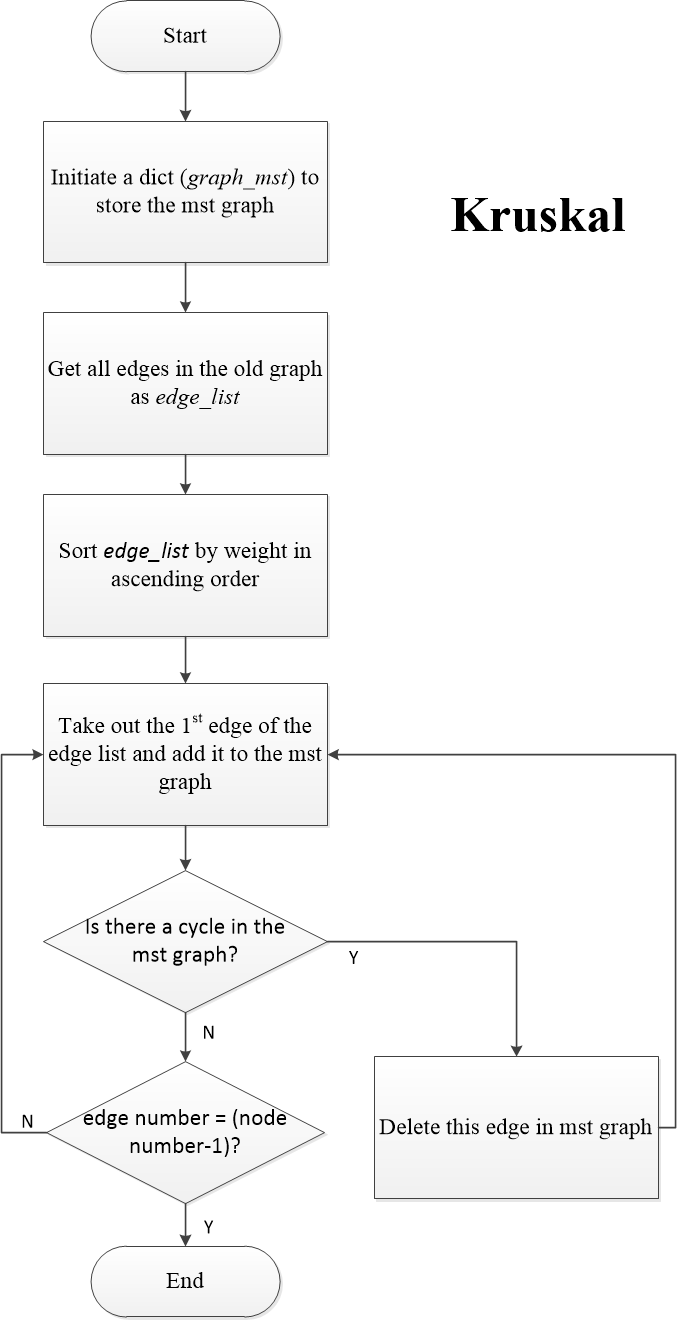
\includegraphics[width=0.8\linewidth, height=24cm]{figures\\flowchartKruskal.png}
            \caption{Flowchart-Kruskal}
            \label{fig:flowchart of Kruskal}
        \end{figure}

        \begin{figure}[H]
            \centering
            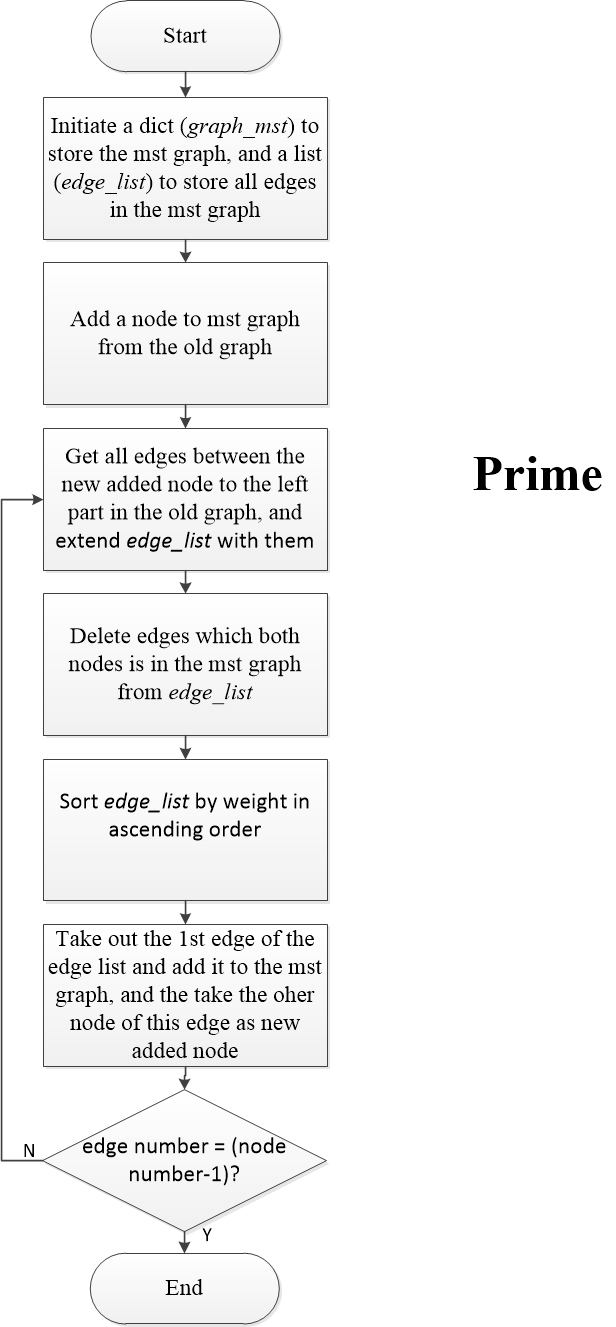
\includegraphics[width=0.8\linewidth, height=24cm]{figures\\flowchartPrime.png}
            \caption{Flowchart-Prime}
            \label{fig:flowchart of Prime}
        \end{figure}

        \begin{figure}[H]
            \centering
            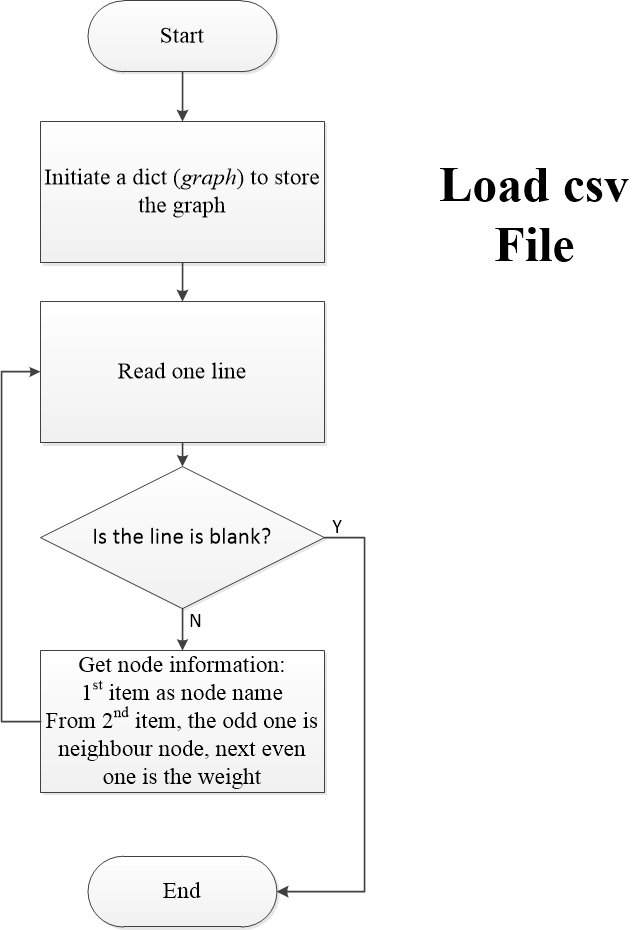
\includegraphics[width=0.8\linewidth, height=24cm]{figures\\flowchartLoadcsv.png}
            \caption{Flowchart-Load csv file}
            \label{fig:flowchart of Load csv}
        \end{figure}

        \begin{figure}[H]
            \centering
            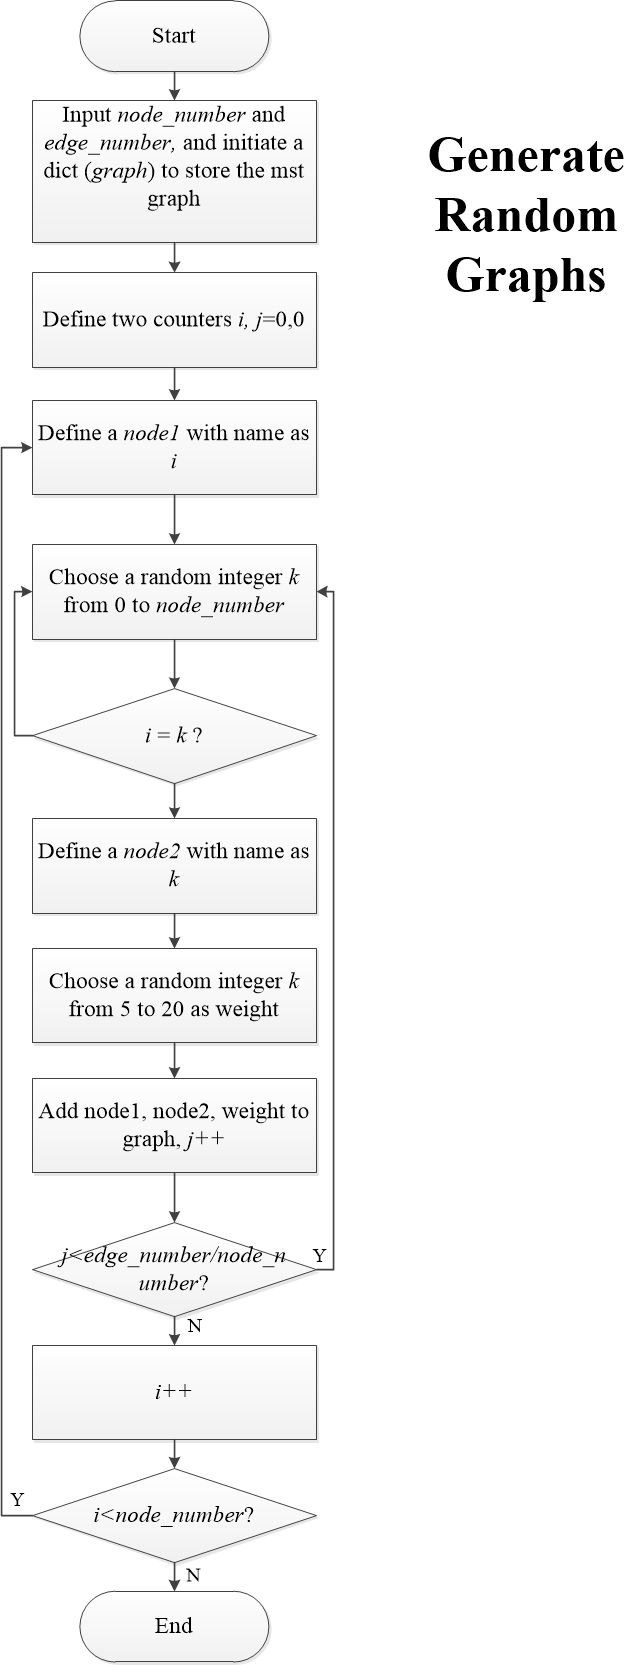
\includegraphics[width=0.8\linewidth, height=24cm]{figures\\flowchartGenerateRandomGraphs.png}
            \caption{Flowchart-Generate Random Graphs}
            \label{fig:flowchart of Generate Random Graphs}
        \end{figure}


    \item Descriptions:
        \begin{itemize}
            \item Kruskal:
                \begin{enumerate}
                    \item Get all edges from the old graph
                    \item Sort edge list by weight in ascending order
                    \item Take out the 1st edge of the edges and add it to the mst graph
                    \item Judge if there are cycles in mst graph, if so, delete it
                    \item judge if the number of edges is enough (node number -1 ), if so, we already get the result, else, back to step3
                \end{enumerate}
            \item Prime:
                \begin{enumerate}
                    \item Add a node to mst graph from the old graph
                    \item Get all edges between the new added node to the left part in the old graph, and extend edge list with them
                    \item Delete edges which both nodes is in the mst graph from edge list
                    \item Sort edge list by weight in ascending order
                    \item Take out the 1st edge of the edge list and add it to the mst graph, and the take the oher node of this edge as new added node
                    \item judge if the number of edges is enough (node number -1 ), if so, we already get the result, else, back to step2
                \end{enumerate}
        \end{itemize}
\end{itemize}
\section{Test and Validate your Code}

% Test Evidence
% Show relevant evidence of testing the functionality of the code
% Any csv files used should be included in the appendix and referred to in your evidence

% Verification
% show that your two algorithms work correctly by comparing your model's solution with a dry run of each algorithm
% you may wish to include trace tables here to show how the program operates



% Summary of key findings
% a short conclusion summarising the main findings of the model

% Appraisal
% For each specification point, explain how your program meets the criteria
% You could refer to any relevant tests here

% System Limitations
% Briefly describe and justify the limitations of the model

% Future Improvements
% Briefly describe how the model could be improved in the future if you had more time.
% Try to include an idea of how this could be implemented.

\section{Summarise and Evaluate}


\begin{itemize}
    \item Conclusion:
    \begin{enumerate}
        \item When node number is a constant, the time cost of kruskal increases with the increase of edge 
        number, while the time cost of prime is basically static
        \item  When edge number is a constant, the time cost of kruskal waves greatly with the increase of node 
        number, while the time cost of prime is basically static
    \end{enumerate}
    \item System Limitations:
        \begin{enumerate}
            \item The interaction to the user is not convenient enough
            \item The show of the result is not visual
        \end{enumerate}
    \item Future Improvements
        \begin{enumerate}
            \item Build gui interface to make it esaier for user to load csv file and get the result
            \item Generate gif pictures to show the solving process of the algorithm
        \end{enumerate}
\end{itemize}

% BIBLIOGRAPHY - REQUIRED IEEE STYLE
\bibliographystyle{IEEEtran}
% add entries to the references.bib file and use the \vite{} command in your document
\bibliography{references}


% APPENDICES (if required)
\clearpage
\appendix % starts the appendix sections
\renewcommand{\appendixpage}{\normalsize\textbf{Appendices}} % change the default style of 

\appendixpage % make the Appendices title appear on the page
\counterwithin{figure}{section} % make figures follow appendix numbering

% this is the title for this part of your appendix
\section{Python code: full listing}
\label{app:app-1}
\lstinputlisting[style=python-code,caption=Automatic Accountant Solution]{listings/automatic_accountant_solution.py}

\newpage
\section{Csv files}
\label{app:app-2}
\lstinputlisting[style=console-output,caption=test\_graph.csv]{listings/test_graph.csv}

\end{document}
